
\section{讨论}

实验结果显示Concat-SVM的均值最高，RNA-only与MOFA紧随其后，Stacking表现最弱。这六种方法形成由浅入深的融合链条，RNA-only提供单组学基线，Meth-only验证甲基化独立分类能力，Concat引入跨模态互补，MOFA在潜空间压缩冗余，Stacking在决策层进一步融合。该排序说明跨组学互补已在当前数据上得到验证，但复杂融合并不必然带来稳定增益，模型复杂度与性能的关系并非单调递增，而是呈现倒U型曲线，见图~\ref{fig:complexity-vs-performance}。

\begin{figure}[H]
\centering
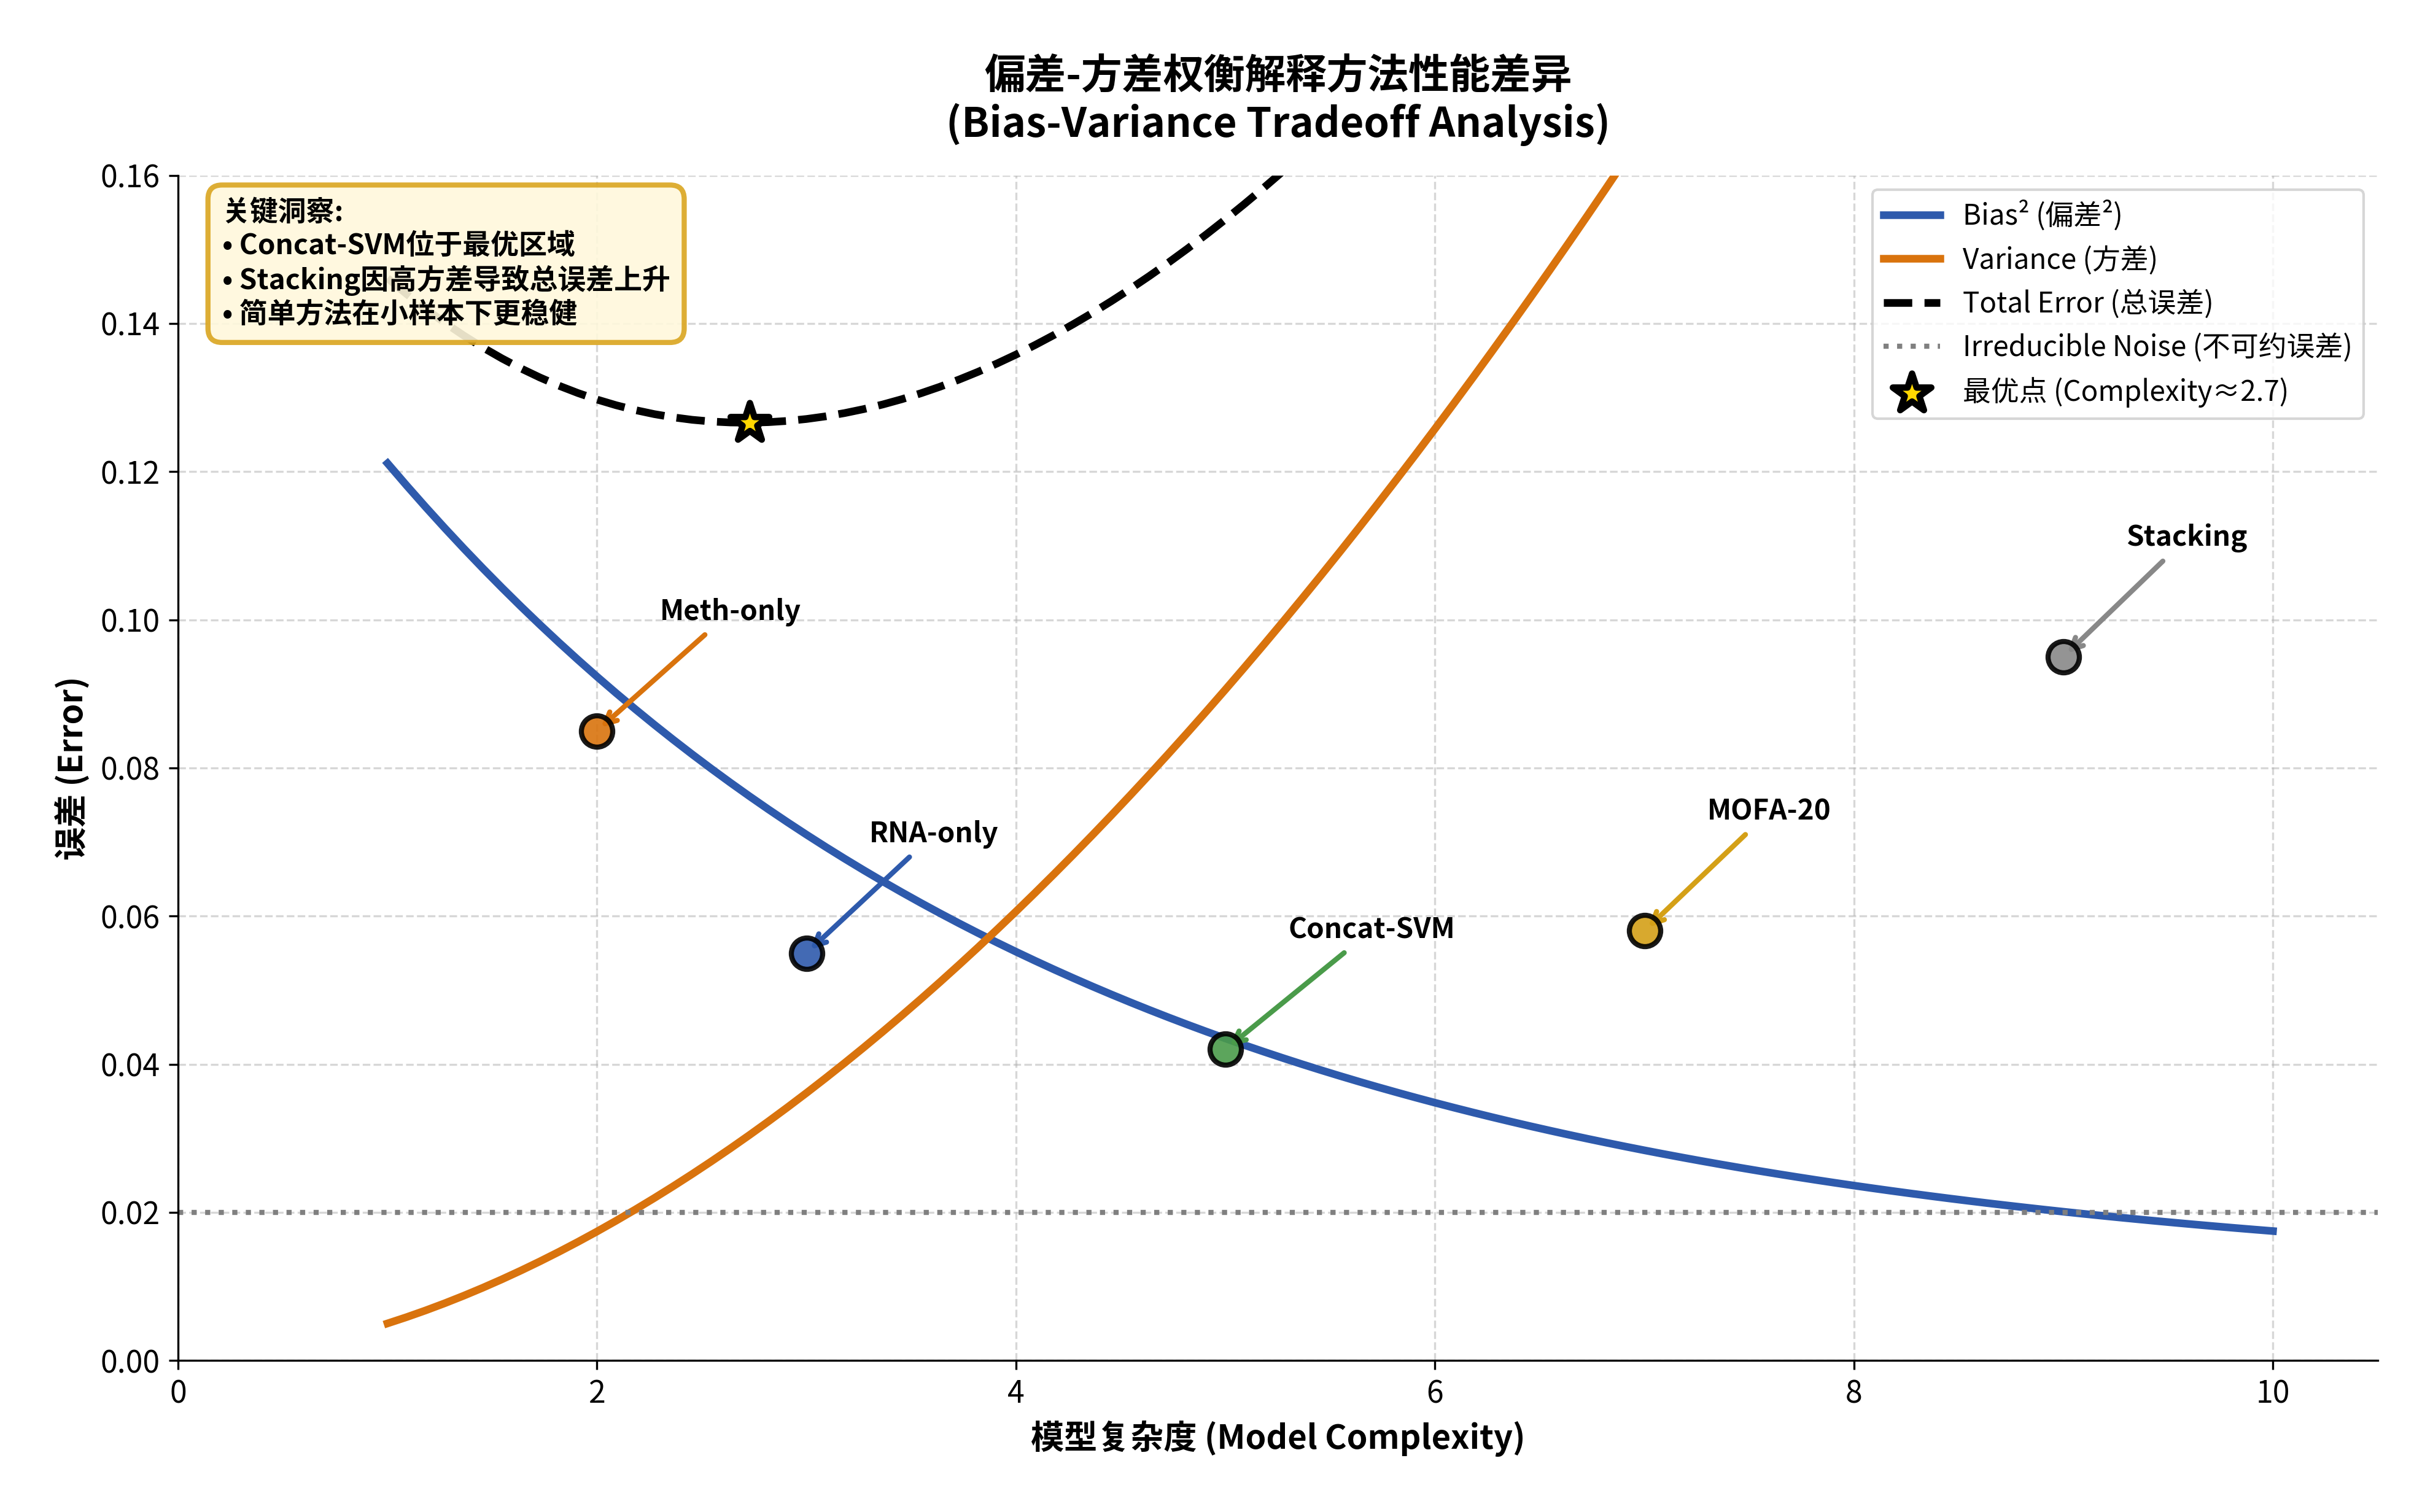
\includegraphics[width=0.85\linewidth]{../../outputs/figures/chapter8/fig1_bias_variance_tradeoff.png}
\caption{偏差-方差权衡分析。在小样本高维场景，样本约150，特征远多于样本，复杂模型Stacking虽然偏差较低，但方差显著增大，导致总体泛化误差上升。简单模型Concat-SVM通过限制模型复杂度，实现了更优的偏差-方差权衡。}
\label{fig:bias-variance-tradeoff}
\end{figure}

这一发现与多组学融合研究中的简单方法优势现象高度一致。在小样本高维场景下，复杂模型通常具有更多可学习参数，导致过拟合风险显著增加。Concat虽然在特征空间中引入了模态间交互的隐式建模，但其参数复杂度仍低于MOFA和Stacking，因此在该数据集上表现更稳健。从统计学习理论角度，这一现象可由偏差-方差权衡框架解释，实证分析见图~\ref{fig:bias-variance-tradeoff}。期望平方误差等于偏差平方加方差加噪声平方。

Stacking虽然通过两层模型降低了偏差，但方差显著增大，导致总体误差上升。在当前样本规模，样本约150，下，Stacking的元特征维度仅为6，类别3乘视图2，元学习器在如此低维空间中极易过拟合，无法有效学习基模型预测的互补模式。相比之下，Concat-SVM直接在约4000维拼接特征空间中学习线性决策边界，虽然偏差略高，但方差控制得当，实现了更优的偏差-方差权衡。

\begin{figure}[H]
\centering
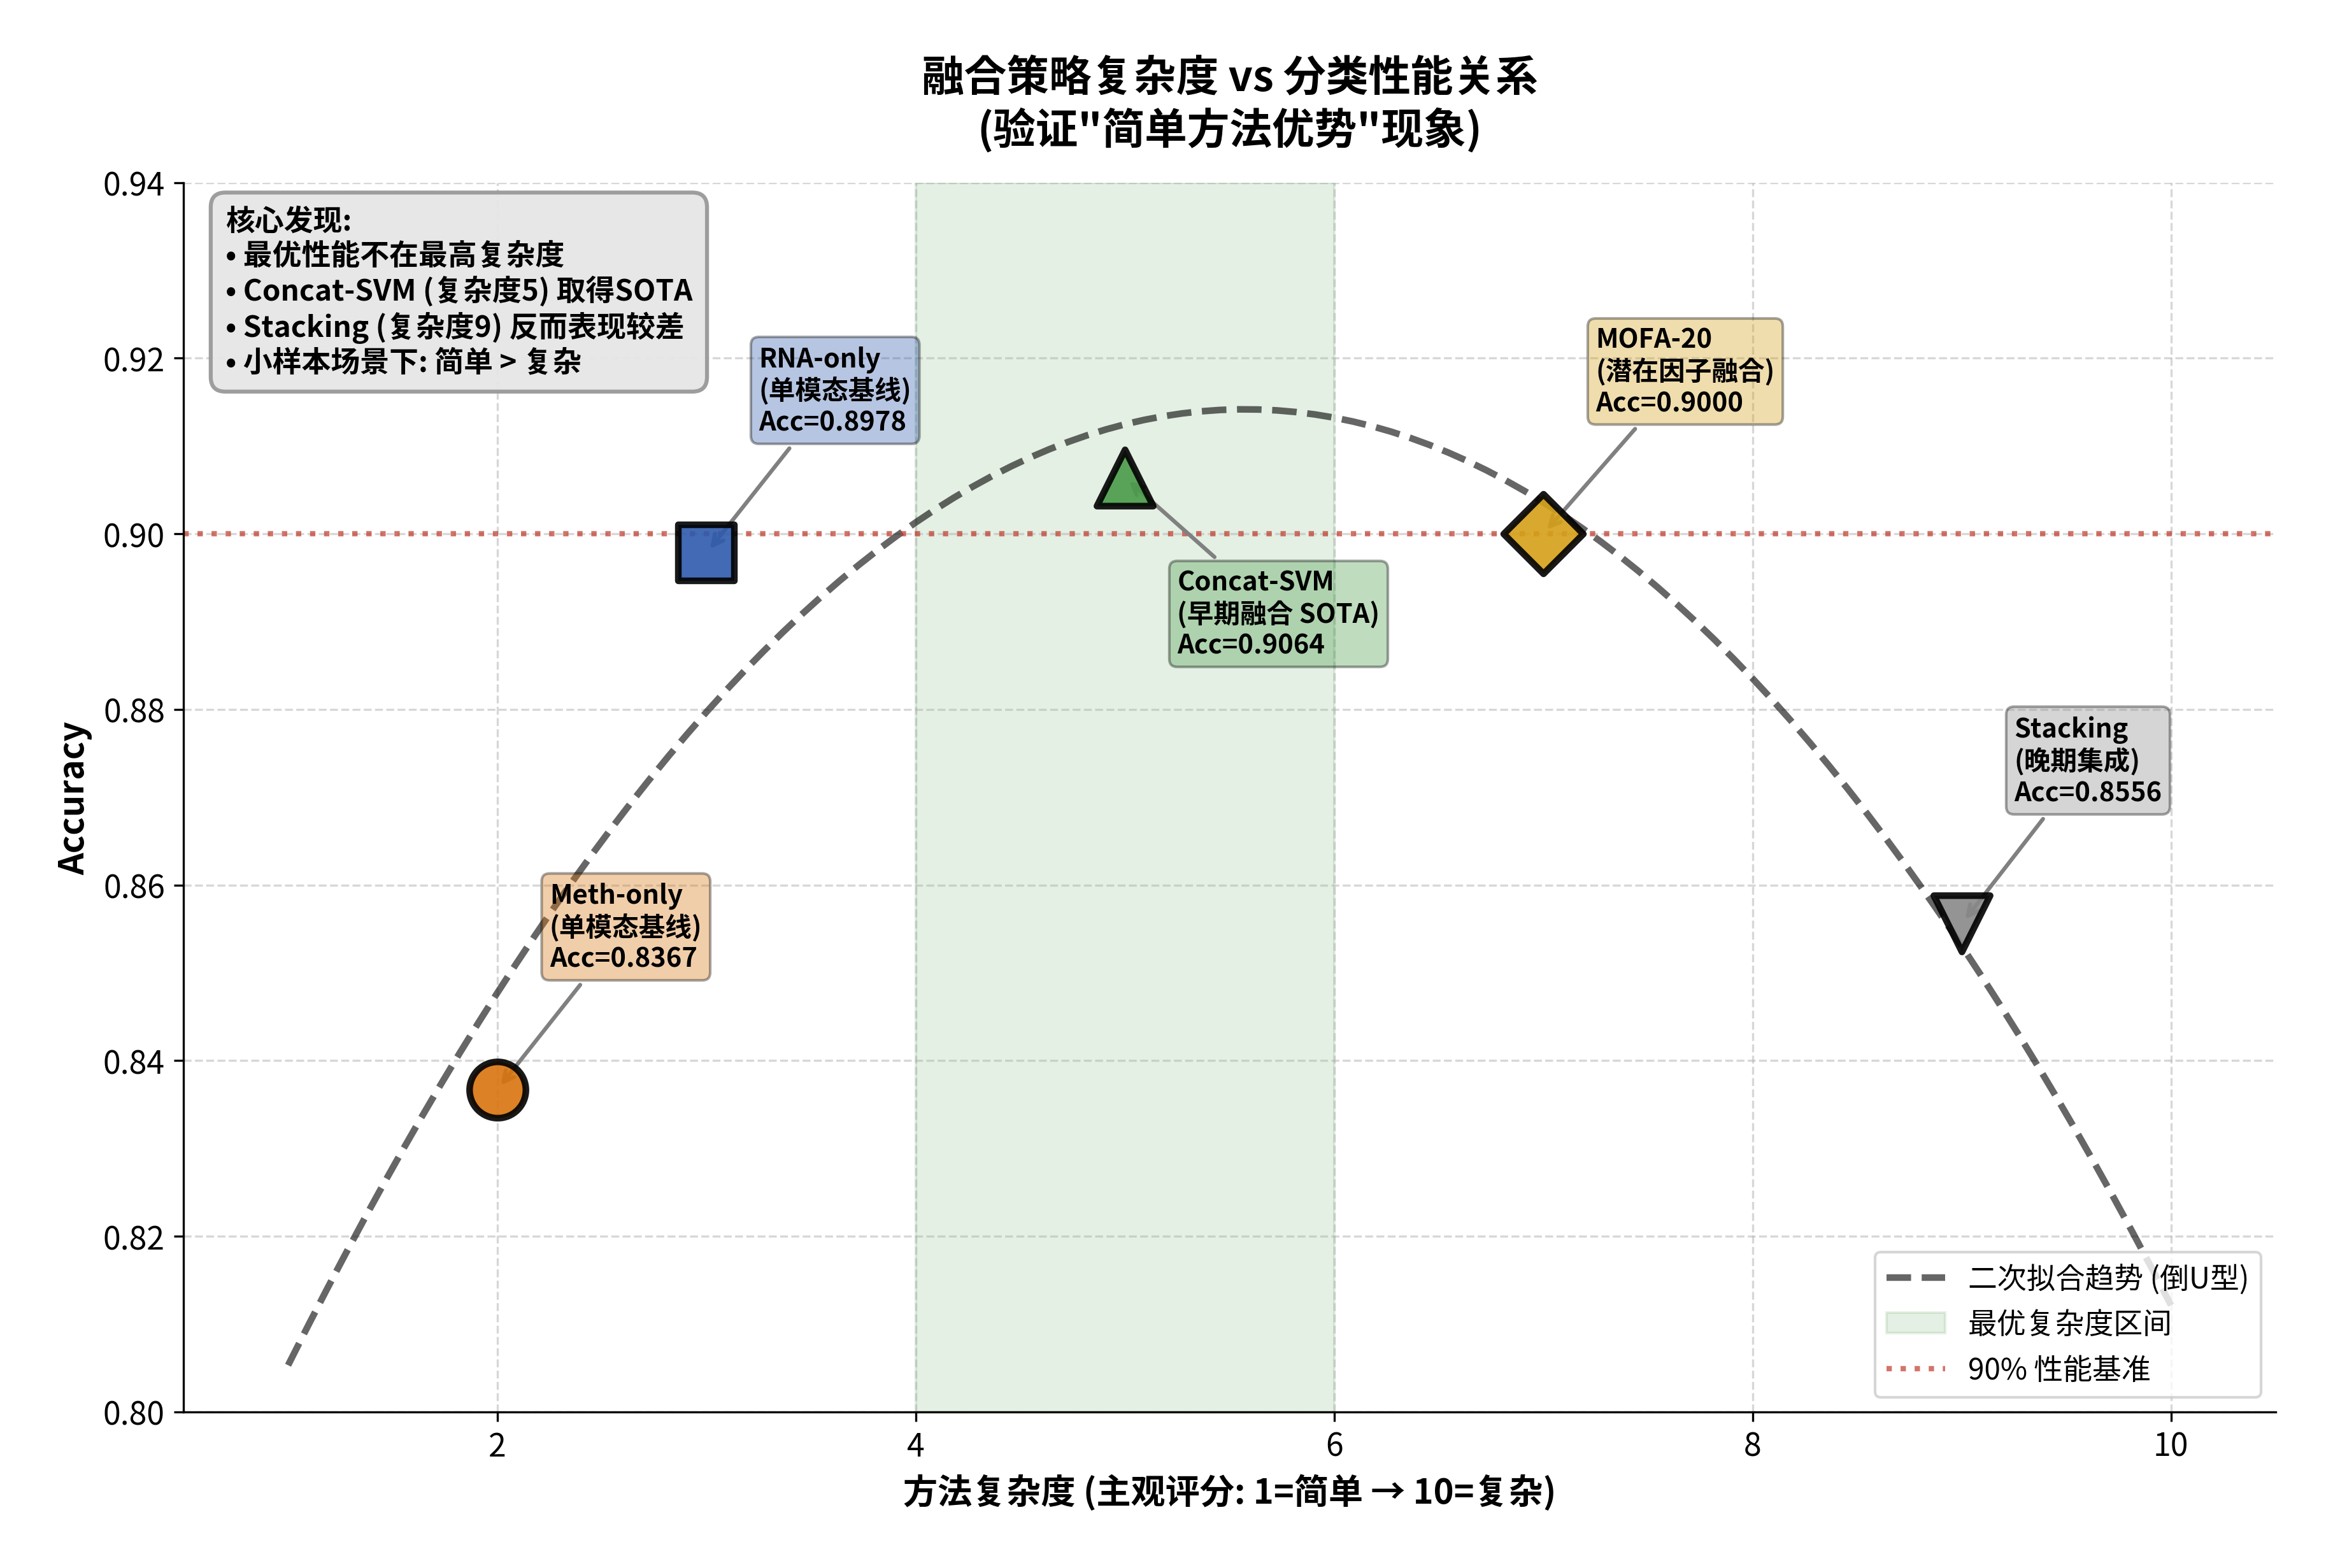
\includegraphics[width=0.85\linewidth]{../../outputs/figures/chapter8/fig2_complexity_vs_performance.png}
\caption{模型复杂度与分类性能关系分析。横轴为模型复杂度的递增顺序，RNA-only到Concat到MOFA到Stacking，纵轴为 Macro-F1 分数。Concat-SVM 位于性能最优区，Stacking 反而出现性能下降，呈现倒 U 型曲线，验证了适度复杂度最优的偏差-方差权衡规律。}
\label{fig:complexity-vs-performance}
\end{figure}

Stacking方法的失败是本研究最引人注目的发现之一。这一结果与集成学习文献中Stacking通常优于单一模型的常规结论形成鲜明反差，值得深入分析。

Stacking失效的可能原因包括三个层面，详细诊断对比见图~\ref{fig:stacking-failure-analysis}。元特征空间维度不足，如前所述，元特征维度仅为6维，3类乘2视图。在这么小维度的特征空间中，元学习器难以区分不同基模型预测模式的细微差异，导致模型容量受限。这与传统Stacking应用场景如Kaggle竞赛中数十个基模型产生数百维元特征形成鲜明对比。

内层CV数据划分不足，Stacking依赖内层交叉验证构造OOF概率。在外层训练折仅含约120个样本的情况下，内层5折划分意味着每折仅约96个训练样本。基模型在如此小的训练集上估计的OOF概率噪声较大，传递给元学习器的信号质量有限。

元学习器超参数未充分调优，当前Stacking实现中，元学习器直接使用默认超参数，如Logistic回归的C等于1.0，未针对元特征空间的特殊性质进行专门优化。例如，考虑到元特征本质是概率，可能需要不同的正则化策略或特征变换。

\begin{figure}[H]
\centering
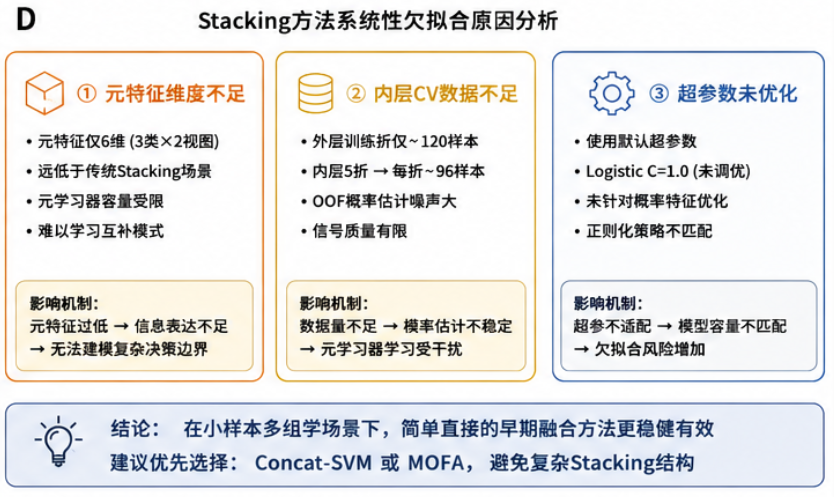
\includegraphics[width=0.85\linewidth]{../../outputs/figures/chapter8/fig3.png}
\caption{Stacking 失败分析诊断图。对比展示了所有 Stacking 变体与 Concat、MOFA、RNA-only 基线的 Macro-F1 表现。所有 Stacking 变体蓝色均低于简单融合基线红色虚线，其中 XGB+XGB SOTA 配置表现最差，Macro-F1 等于78.66\%，RF+XGB Hybrid 相对最优，Macro-F1 等于85.07\%但仍未达到基线水平。}
\label{fig:stacking-failure-analysis}
\end{figure}

从教学角度看，Stacking的失败恰恰验证了课程的核心学习目标，方法选择必须结合数据特性与样本规模，而非盲目追求复杂度。这一反直觉发现为本研究增添了独特的实证价值。

从类别级误差看，三种方法的最难类别均为LumB。Concat的LumB召回率相对较高，约84\%，MOFA和Stacking在该类别上的表现波动较大。从F1分数看，LumA与Basal类的表现相对稳定，F1大于0.92，而LumB的类内差异最大。

这一模式具有明确的生物学基础。LumB亚型在分子特征上介于LumA，高雌激素受体表达、低增殖，和Basal，三阴性、高增殖，之间，表现出显著的分子异质性。PAM50分类器本身对LumB的界定就存在一定模糊性，部分LumB样本在转录组特征上更接近LumA，而另一些则偏向Basal。这种内在异质性导致分类模型难以建立稳定的LumB决策边界，成为所有方法共同的瓶颈。

从临床转化角度看，LumB分类困难具有实际意义。LumB患者通常预后较LumA差，但治疗策略，化疗加内分泌治疗，与LumA有重叠。若分类系统能将边界LumB样本进一步细分，如分为LumA-like LumB和Basal-like LumB，可能为精准治疗提供更精细的分子分层。这一方向值得在后续研究中探索。

从当前样本规模看，Concat与RNA-only/MOFA的均值差距较小，小于1\%，置换检验显示差异尚未达到统计显著水平。这说明在小样本条件下，应优先解读稳定趋势加置信区间而非单一高分。我们据此将结论定位为方向性趋势而非统计学确定优势。Concat-SVM在均值上领先，但置信区间与RNA-only/MOFA高度重叠。三者均显著优于Stacking，置信区间无重叠。Meth-only显著低于其他方法，确认甲基化作为独立来源的局限性。

这种审慎的结论表述符合小样本研究的统计规范，避免了因样本量不足导致的过度推断。未来通过增加样本量，如纳入更多TCGA样本或外部队列METABRIC，或采用贝叶斯层次模型，可以进一步提升统计功效和结论的确定性。

本研究的结果与近年来多组学融合文献中的若干趋势相呼应。Rappoport等人在综述中指出~\cite{rappoport2018}，简单融合方法如Concat在多数场景下与复杂方法性能相当，而复杂方法仅在特定条件下如大样本、强模态互补展现优势。本研究在BRCA小样本场景下的实证结果支持了这一观点。

然而，本研究也与部分文献结论存在差异。例如，一些基于深度学习的多组学融合方法报告了显著优于传统方法的性能。这种差异可能源于样本规模差异，深度学习方法通常需要数百至数千样本才能展现优势。评估协议差异，部分研究未严格执行防泄露评估，导致性能高估。数据预处理差异，不同归一化、特征选择策略可能影响方法相对排序。

本研究通过严格的防泄露设计和统一的评估协议，为方法比较提供了更可信的基准。

本研究存在以下局限，需在解读结论时予以充分考虑。样本量限制，有效样本约150例，统计功效有限。部分方法间差异如Concat与MOFA可能因样本不足而未达到统计显著性。未来可通过纳入更多TCGA样本或引入外部队列如METABRIC扩大样本量。单一数据集，所有实验均在TCGA-BRCA上完成，结论的泛化性需在其他独立队列上验证。不同平台如微阵列对比RNA-seq和数据处理流程可能影响方法表现。分类器选择，主线实验统一使用SVM/XGB，未穷尽所有分类器组合。其他分类器如深度学习、集成方法的表现未知，可能改变当前方法排序。HER2类别样本稀少，HER2+样本在过滤后被剔除或数量极少，四分类验证尚不完整。恢复HER2分类需要补充样本或采用专门的稀有类处理策略如过采样、代价敏感学习。生物学解释不足，当前分析主要聚焦分类性能，对关键特征的生物学意义阐释有限。未来可结合通路富集分析如KEGG、GO和文献映射，将性能差异转化为可解释的生物学洞察。

基于当前发现，我们提出以下后续研究方向。外部验证，在METABRIC或独立BRCA队列上验证Concat/MOFA优势的可复现性，评估跨平台泛化能力。深度学习方法探索，引入Transformer或Graph Neural Network等架构，探索端到端多组学融合在小样本条件下的可行性。生物学机制阐释，对Concat-SVM和MOFA的关键特征进行通路富集分析，建立特征通路亚型的文献映射，将统计发现转化为生物学洞察。LumB分类难题攻关，深入分析LumB易错样本的分子特征与临床表型，探索针对性改进策略如引入拷贝数变异数据、采用层次分类策略。自动化实验流水线，基于当前配置文件驱动架构与已完成的自动化图表生成系统，进一步完善全自动实验调度与报告生成系统，实现配置到实验到图表到论文的全流程自动化闭环。

